% Created 2019-09-05 jue 11:37
\documentclass[letterpaper,fleqn]{scrartcl}
\usepackage[utf8]{inputenc}
\usepackage[T1]{fontenc}
\usepackage{fixltx2e}
\usepackage{graphicx}
\usepackage{longtable}
\usepackage{float}
\usepackage{wrapfig}
\usepackage{rotating}
\usepackage[normalem]{ulem}
\usepackage{amsmath}
\usepackage{textcomp}
\usepackage{marvosym}
\usepackage{wasysym}
\usepackage{amssymb}
\usepackage{hyperref}
\tolerance=1000
\usepackage{khpreamble}
\usepackage{tabularx}
\usepackage{geometry}
\usepackage{pgfplots}
\pgfplotsset{compat=1.13}
\geometry{top=20mm, bottom=20mm, left=24mm, right=18mm}
\author{Kjartan Halvorsen}
\date{}
\title{Pole-placement exercise}
\hypersetup{
  pdfkeywords={},
  pdfsubject={},
  pdfcreator={Emacs 25.3.50.2 (Org mode 8.2.10)}}
\begin{document}

\maketitle

\section*{Plot the poles}
\label{sec-1}
\begin{center}
\textbf{s-plane} \hspace*{0.4\linewidth} \textbf{z-plane}\\
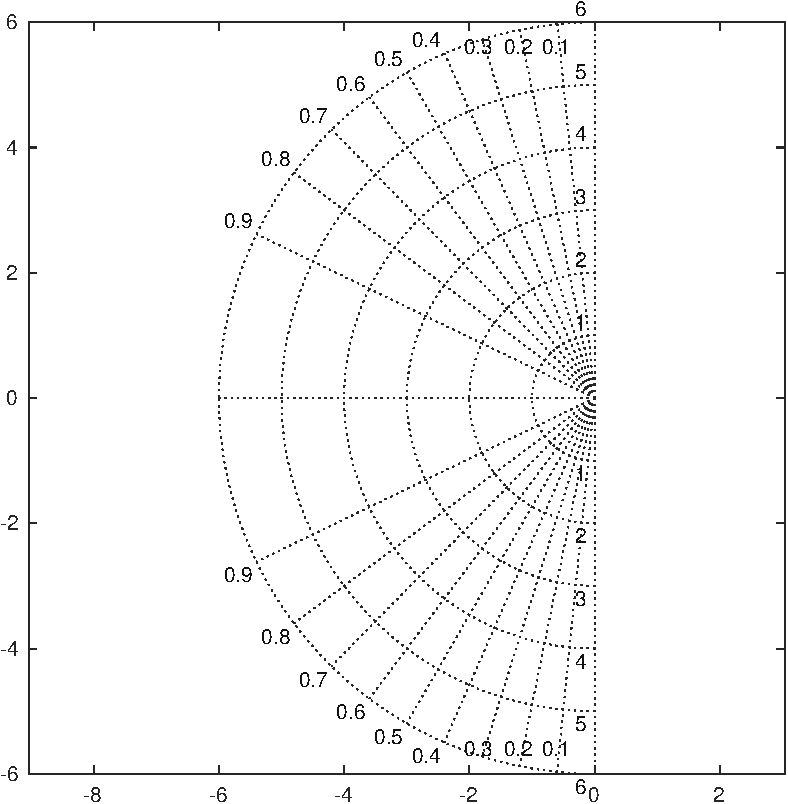
\includegraphics[height=0.34\textheight]{../../figures/sgrid-crop} \hspace*{3mm}
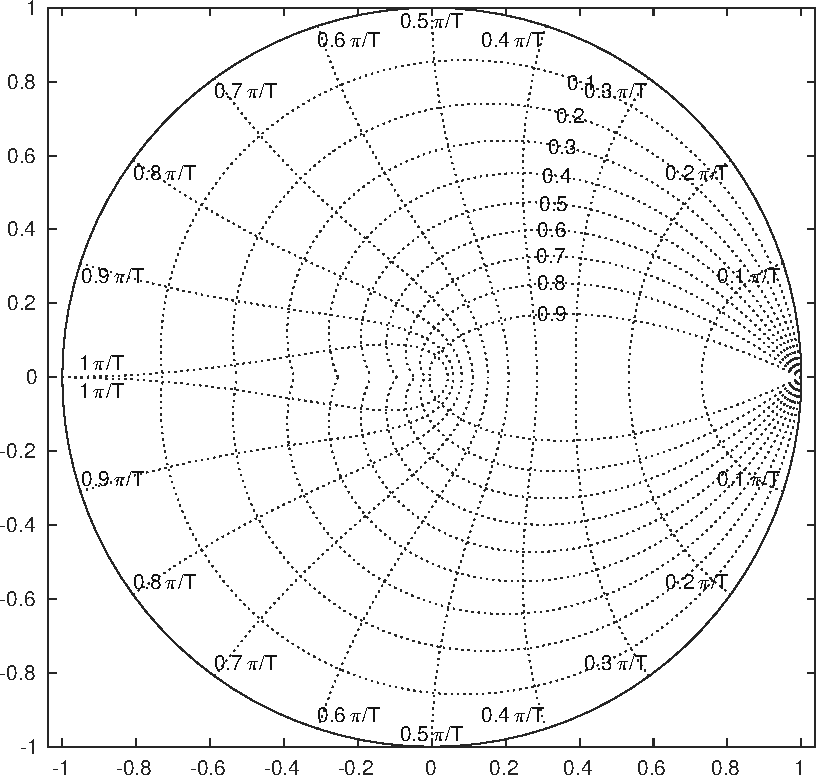
\includegraphics[height=0.34\textheight]{../../figures/zgrid-crop}\\
\end{center}

Plot the poles of the following closed-loop discrete-time systems (as crosses in the z-plane). Plot also the corresponding continous-time poles (in the s-plane) using the sampling period \(h=0.2\). Rank the systems from 1 to 5 according to how desirable the performance of each system is.
\begin{description}
\item[{a}] \( G_c(z) = \frac{0.026z + 0.024}{z(z-0.95)}\)
\item[{b}] \( G_c(z) = \frac{0.13z + 0.12}{z^2 - z + 0.25} \)
\item[{c}] \(G_c(z) = \frac{0.54z + 0.52}{(z-0.5)^2 + 0.81}\)
\item[{d}] \(G_c(z) = \frac{0.025z + 0.025}{(z-0.8)^2 - 0.09}\)
\item[{e}] \(G_c(z) = \frac{0.068z + 0.062}{(z-0.8)^2 + 0.09}\)
\end{description}

\newpage 


\section*{Pole placement and step response}
\label{sec-2}
Pair each of the discrete-time systems in the previous exercise with the correct step response below.
\begin{center}
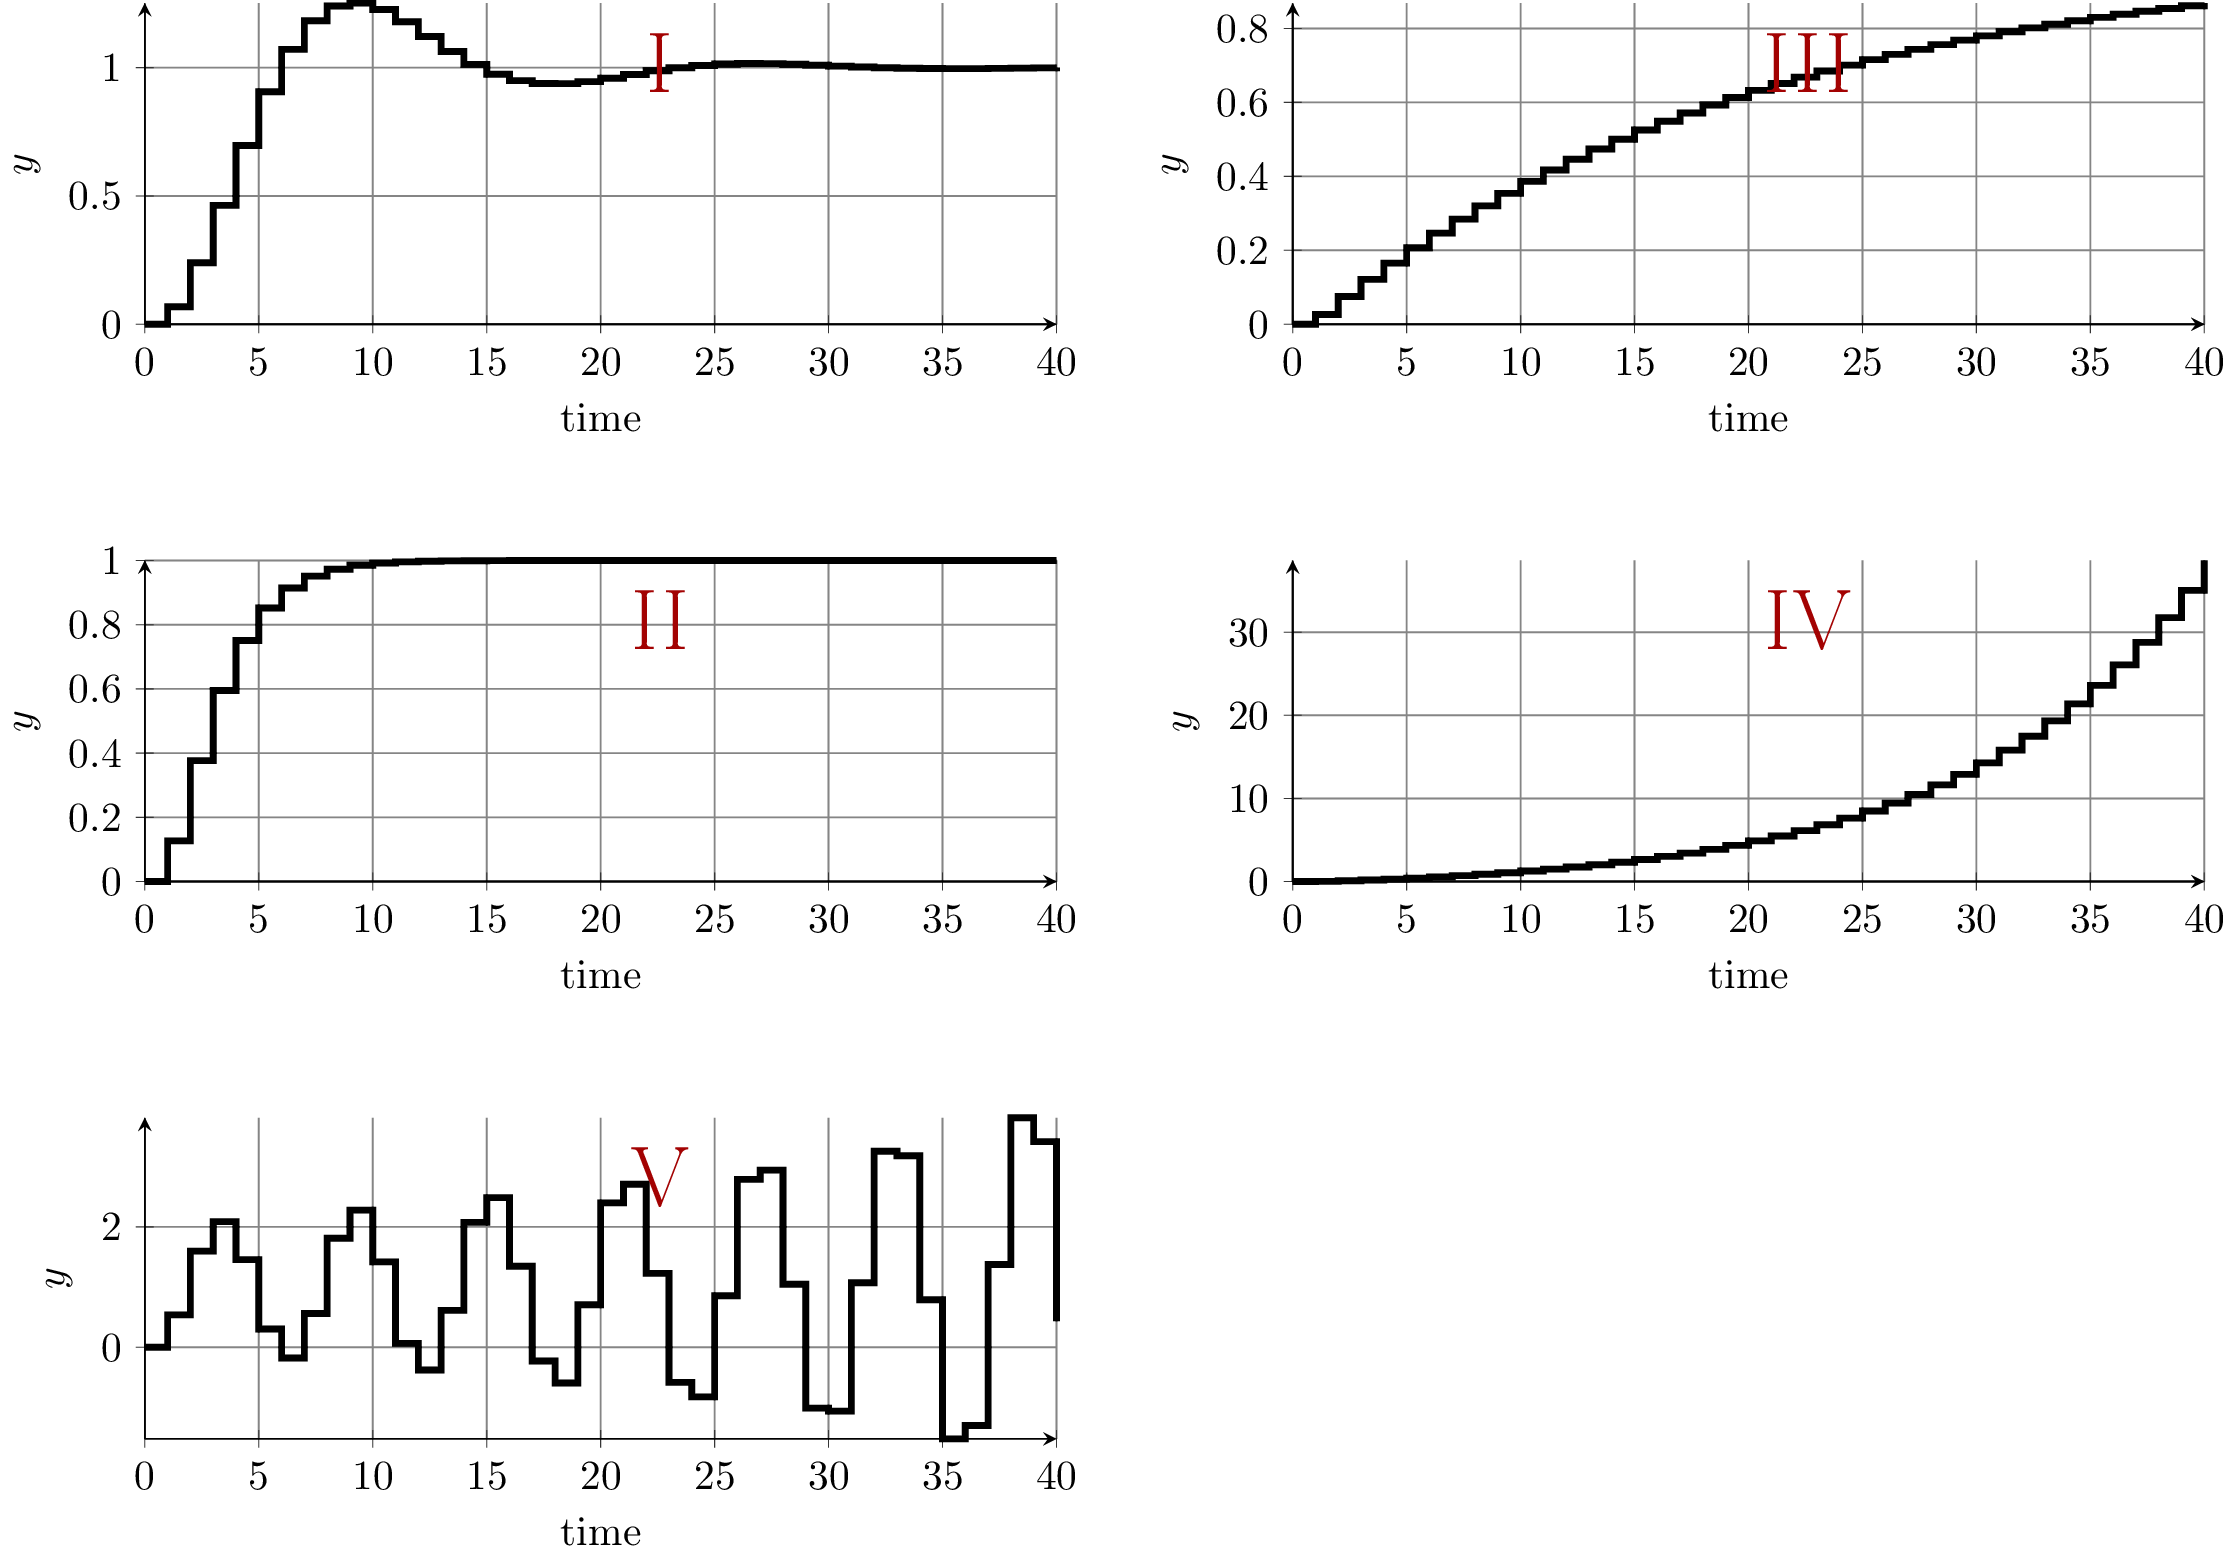
\includegraphics[width=\linewidth]{../../figures/closed-loop-step-responsen}
\end{center}
% Emacs 25.3.50.2 (Org mode 8.2.10)
\end{document}